\documentclass{article}

\usepackage{fullpage}
\usepackage{amsmath}
\usepackage{amssymb}
\usepackage{amsthm}
\usepackage{graphicx}
\usepackage{xcolor}
\usepackage{hyperref}

\newcounter{placeholderCount}
\newcommand{\placeholder}[1]{{
    \stepcounter{placeholderCount}
    \color{red} [#1]
}}

\newcounter{solutionCount}
\newcommand{\solution}[1]{
    \stepcounter{solutionCount}
    \paragraph{Solution \thesolutionCount.}
    {
        #1
    }
}

\title{
    Deep Learning (Spring 2026) \\
    Solution for Assignment 4
}
\author{
    Pan Changxun
    \\
    2024011323
}

\begin{document}

\maketitle

%% Problem 1
\solution{
    \textbf{False.}

    $\mathrm{KL}(q_\theta \| p)$ is the \emph{exclusive} (reverse) KL divergence:
    \[
      \mathrm{KL}(q_\theta \| p) = \int q_\theta(x) \log \frac{q_\theta(x)}{p(x)} \, dx.
    \]
    Whenever $q_\theta(x) > 0$ but $p(x) \approx 0$, the integrand blows up, so the optimizer avoids placing mass where $p$ has no support. However, wherever $p(x) > 0$ but $q_\theta(x) = 0$, the integrand contributes $0$ (weighted by $q_\theta$), so there is \emph{no} penalty for missing modes. Therefore, minimizing $\mathrm{KL}(q_\theta \| p)$ produces a \emph{mode-seeking} distribution: $q_\theta$ concentrates on one (typically the dominant) mode of $p$ rather than uniformly covering all modes. The mode-covering behavior would instead correspond to minimizing $\mathrm{KL}(p \| q_\theta)$ (the inclusive / forward KL).
}

%% Problem 2
\solution{
    \textbf{True.}

    In VAE, the latent variable $z$ is sampled from the encoder distribution $q_\phi(z|x)$. This sampling operation is not differentiable, which blocks gradient flow back to the encoder parameters $\phi$. The reparameterization trick rewrites $z = \mu_\phi(x) + \sigma_\phi(x) \odot \epsilon$, where $\epsilon \sim \mathcal{N}(0, I)$, so that the stochasticity is moved to $\epsilon$ which does not depend on $\phi$. This makes $z$ a deterministic, differentiable function of $\phi$, enabling gradients to pass back to the encoder.
}

%% Problem 3
\solution{
    \textbf{False.}

    The exact posterior $p(z|x) = \frac{p(x|z)p(z)}{p(x)}$ requires computing the marginal likelihood $p(x) = \int p(x|z)p(z)\,dz$, which is generally intractable for complex models (e.g., when $p(x|z)$ is parameterized by a neural network). This intractability is precisely the reason VAE introduces a variational approximation $q_\phi(z|x)$ to approximate the true posterior.
}

%% Problem 4
\solution{
    \textbf{False.}

    In $\beta$-VAE, the objective is:
    \[
      \mathcal{L} = \mathbb{E}_{q_\phi(z|x)}[\log p_\theta(x|z)] - \beta \, \mathrm{KL}(q_\phi(z|x) \| p(z)).
    \]
    A large $\beta$ puts more weight on the KL term, which pushes $q_\phi(z|x)$ closer to the prior $p(z) = \mathcal{N}(0, I)$. Since the prior has independent (uncorrelated) dimensions, a large $\beta$ enforces the latent variables to be more \emph{independent} (disentangled) from each other, not correlated.
}

%% Problem 5 (EM Algorithm)
\solution{
    We need to show that alternating maximization of $\mathcal{F}(\theta, q) = \mathbb{E}_{z \sim q}[\log p_\theta(x,z)] + H(q)$ is equivalent to the EM algorithm.

    \textbf{E-step:} We show $q^{(t)} = \arg\max_q \mathcal{F}(\theta^{(t)}, q)$ gives $q^{(t)}(z) = p_{\theta^{(t)}}(z|x)$.

    Rewrite $\mathcal{F}$:
    \begin{align}
    \mathcal{F}(\theta, q)
    &= \mathbb{E}_{z \sim q}[\log p_\theta(x,z)] + H(q) \nonumber \\
    &= \sum_z q(z) \log p_\theta(x,z) - \sum_z q(z) \log q(z) \nonumber \\
    &= \sum_z q(z) \log \frac{p_\theta(x,z)}{q(z)} \nonumber \\
    &= \sum_z q(z) \log \frac{p_\theta(z|x) \, p_\theta(x)}{q(z)} \nonumber \\
    &= \sum_z q(z) \log \frac{p_\theta(z|x)}{q(z)} + \log p_\theta(x) \nonumber \\
    &= -\mathrm{KL}(q(z) \| p_\theta(z|x)) + \log p_\theta(x). \label{eq:F-rewrite}
    \end{align}

    Since $\log p_\theta(x)$ does not depend on $q$, maximizing $\mathcal{F}(\theta^{(t)}, q)$ over $q$ is equivalent to minimizing $\mathrm{KL}(q \| p_{\theta^{(t)}}(z|x))$. The KL divergence is non-negative and equals zero if and only if $q(z) = p_{\theta^{(t)}}(z|x)$. Therefore:
    \[
      q^{(t)}(z) = p_{\theta^{(t)}}(z|x).
    \]
    This is exactly the E-step of EM, which computes the posterior $p_{\theta^{(t)}}(z|x)$.

    \bigskip
    \textbf{M-step:} We show $\theta^{(t+1)} = \arg\max_\theta \mathcal{F}(\theta, q^{(t)})$ is equivalent to $\arg\max_\theta Q(\theta|\theta^{(t)})$.

    With $q^{(t)}(z) = p_{\theta^{(t)}}(z|x)$ fixed:
    \begin{align}
    \mathcal{F}(\theta, q^{(t)})
    &= \mathbb{E}_{z \sim q^{(t)}}[\log p_\theta(x,z)] + H(q^{(t)}) \nonumber \\
    &= \mathbb{E}_{z \sim p_{\theta^{(t)}}(z|x)}[\log p_\theta(x,z)] + H(q^{(t)}). \nonumber
    \end{align}

    Since $H(q^{(t)})$ does not depend on $\theta$:
    \[
      \arg\max_\theta \mathcal{F}(\theta, q^{(t)}) = \arg\max_\theta \mathbb{E}_{z \sim p_{\theta^{(t)}}(z|x)}[\log p_\theta(x,z)] = \arg\max_\theta Q(\theta|\theta^{(t)}).
    \]
    This is exactly the M-step of EM.

    Therefore, the alternating maximization of $\mathcal{F}(\theta, q)$ is equivalent to the EM algorithm. $\hfill\blacksquare$
}

%% Problem 6 (KL-Divergence)
\solution{
    \begin{enumerate}
        \item \textbf{(Gaussian KL Divergence)}

        For two $d$-dimensional Gaussians $\mathcal{N}_0(\mu_0, \Sigma_0)$ and $\mathcal{N}_1(\mu_1, \Sigma_1)$:
        \begin{align}
        \mathrm{KL}(\mathcal{N}_0 \| \mathcal{N}_1)
        &= \mathbb{E}_{x \sim \mathcal{N}_0}\left[\log \frac{p_0(x)}{p_1(x)}\right] \nonumber \\
        &= \mathbb{E}_{x \sim \mathcal{N}_0}[\log p_0(x)] - \mathbb{E}_{x \sim \mathcal{N}_0}[\log p_1(x)]. \nonumber
        \end{align}

        \textbf{First term:}
        \begin{align}
        \mathbb{E}_{x \sim \mathcal{N}_0}[\log p_0(x)]
        &= \mathbb{E}\left[-\frac{d}{2}\log(2\pi) - \frac{1}{2}\log|\Sigma_0| - \frac{1}{2}(x-\mu_0)^T \Sigma_0^{-1}(x-\mu_0)\right] \nonumber \\
        &= -\frac{d}{2}\log(2\pi) - \frac{1}{2}\log|\Sigma_0| - \frac{1}{2}\mathrm{tr}(\Sigma_0^{-1}\Sigma_0) \nonumber \\
        &= -\frac{d}{2}\log(2\pi) - \frac{1}{2}\log|\Sigma_0| - \frac{d}{2}. \nonumber
        \end{align}

        \textbf{Second term:}
        \begin{align}
        \mathbb{E}_{x \sim \mathcal{N}_0}[\log p_1(x)]
        &= \mathbb{E}\left[-\frac{d}{2}\log(2\pi) - \frac{1}{2}\log|\Sigma_1| - \frac{1}{2}(x-\mu_1)^T \Sigma_1^{-1}(x-\mu_1)\right]. \nonumber
        \end{align}

        For the quadratic term, let $x = \mu_0 + \Sigma_0^{1/2}\epsilon$ where $\epsilon \sim \mathcal{N}(0,I)$:
        \begin{align}
        &\mathbb{E}[(x-\mu_1)^T \Sigma_1^{-1}(x-\mu_1)] \nonumber \\
        &= \mathbb{E}[((x-\mu_0)+(\mu_0-\mu_1))^T \Sigma_1^{-1}((x-\mu_0)+(\mu_0-\mu_1))] \nonumber \\
        &= \mathbb{E}[(x-\mu_0)^T\Sigma_1^{-1}(x-\mu_0)] + (\mu_0-\mu_1)^T\Sigma_1^{-1}(\mu_0-\mu_1) \nonumber \\
        &= \mathrm{tr}(\Sigma_1^{-1}\Sigma_0) + (\mu_1-\mu_0)^T\Sigma_1^{-1}(\mu_1-\mu_0). \nonumber
        \end{align}

        where the cross terms vanish because $\mathbb{E}[x - \mu_0] = 0$.

        Therefore:
        \begin{align}
        \mathbb{E}_{x \sim \mathcal{N}_0}[\log p_1(x)]
        &= -\frac{d}{2}\log(2\pi) - \frac{1}{2}\log|\Sigma_1| - \frac{1}{2}\left[\mathrm{tr}(\Sigma_1^{-1}\Sigma_0) + (\mu_1-\mu_0)^T\Sigma_1^{-1}(\mu_1-\mu_0)\right]. \nonumber
        \end{align}

        Subtracting:
        \begin{align}
        \mathrm{KL}(\mathcal{N}_0 \| \mathcal{N}_1)
        &= -\frac{1}{2}\log|\Sigma_0| - \frac{d}{2} + \frac{1}{2}\log|\Sigma_1| + \frac{1}{2}\mathrm{tr}(\Sigma_1^{-1}\Sigma_0) + \frac{1}{2}(\mu_1-\mu_0)^T\Sigma_1^{-1}(\mu_1-\mu_0) \nonumber \\
        &= \frac{1}{2}\left(\mathrm{tr}(\Sigma_1^{-1}\Sigma_0) + (\mu_1-\mu_0)^T\Sigma_1^{-1}(\mu_1-\mu_0) - d + \log\frac{|\Sigma_1|}{|\Sigma_0|}\right). \nonumber
        \end{align}
        $\hfill\blacksquare$

        \item \textbf{(Convexity)}

        We use the log-sum inequality. For any $\lambda \in [0,1]$ and discrete distributions $p_1, p_2, q_1, q_2$ over $\mathcal{Y} = \{1,\ldots,n\}$:

        \begin{align}
        &\mathrm{KL}(\lambda p_1 + (1-\lambda)p_2 \| \lambda q_1 + (1-\lambda)q_2) \nonumber \\
        &= \sum_{y=1}^{n} \left[\lambda p_1(y) + (1-\lambda)p_2(y)\right] \log \frac{\lambda p_1(y) + (1-\lambda)p_2(y)}{\lambda q_1(y) + (1-\lambda)q_2(y)}. \nonumber
        \end{align}

        By the log-sum inequality, for non-negative reals $a_i, b_i$ ($i=1,2$) with $a_1 + a_2 > 0$ and $b_1 + b_2 > 0$:
        \[
        (a_1 + a_2) \log \frac{a_1 + a_2}{b_1 + b_2} \leq a_1 \log \frac{a_1}{b_1} + a_2 \log \frac{a_2}{b_2}.
        \]

        For each $y$, let $a_1 = \lambda p_1(y)$, $a_2 = (1-\lambda)p_2(y)$, $b_1 = \lambda q_1(y)$, $b_2 = (1-\lambda)q_2(y)$. Applying the log-sum inequality:
        \begin{align}
        &[\lambda p_1(y) + (1-\lambda)p_2(y)] \log \frac{\lambda p_1(y) + (1-\lambda)p_2(y)}{\lambda q_1(y) + (1-\lambda)q_2(y)} \nonumber \\
        &\leq \lambda p_1(y) \log \frac{\lambda p_1(y)}{\lambda q_1(y)} + (1-\lambda)p_2(y) \log \frac{(1-\lambda)p_2(y)}{(1-\lambda)q_2(y)} \nonumber \\
        &= \lambda p_1(y) \log \frac{p_1(y)}{q_1(y)} + (1-\lambda)p_2(y) \log \frac{p_2(y)}{q_2(y)}. \nonumber
        \end{align}

        Summing over all $y \in \mathcal{Y}$:
        \begin{align}
        \mathrm{KL}(\lambda p_1 + (1-\lambda)p_2 \| \lambda q_1 + (1-\lambda)q_2)
        &\leq \sum_{y} \lambda p_1(y) \log \frac{p_1(y)}{q_1(y)} + \sum_{y}(1-\lambda) p_2(y) \log \frac{p_2(y)}{q_2(y)} \nonumber \\
        &= \lambda \,\mathrm{KL}(p_1\|q_1) + (1-\lambda)\,\mathrm{KL}(p_2\|q_2). \nonumber
        \end{align}
        $\hfill\blacksquare$

        \item \textbf{(Inclusive/Exclusive KL)}

        The target distribution is $p(x) = \frac{1}{3}\mathcal{N}(-3,1) + \frac{2}{3}\mathcal{N}(3,1)$. We fit $q(x) = \mathcal{N}(\mu, \sigma^2)$.

        \begin{itemize}
            \item \textbf{Inclusive KL} ($\mathrm{KL}(p\|q)$, forward KL): mode-covering. The optimization finds a $q$ that must cover all modes of $p$ (wherever $p(x)>0$, $q(x)$ must be non-zero), resulting in a broad distribution centered between the modes. Result: $\mu \approx 1.00$, $\sigma \approx 3.00$.
            \item \textbf{Exclusive KL} ($\mathrm{KL}(q\|p)$, reverse KL): mode-seeking. The optimization finds a $q$ that concentrates on the dominant mode of $p$ (since $q$ can safely ignore modes). Result: $\mu \approx 3.00$, $\sigma \approx 1.02$.
        \end{itemize}

        We solve both optimizations numerically using gradient descent. The resulting figure is shown in Figure~\ref{fig:kl}.

        \begin{figure}[h]
            \centering
            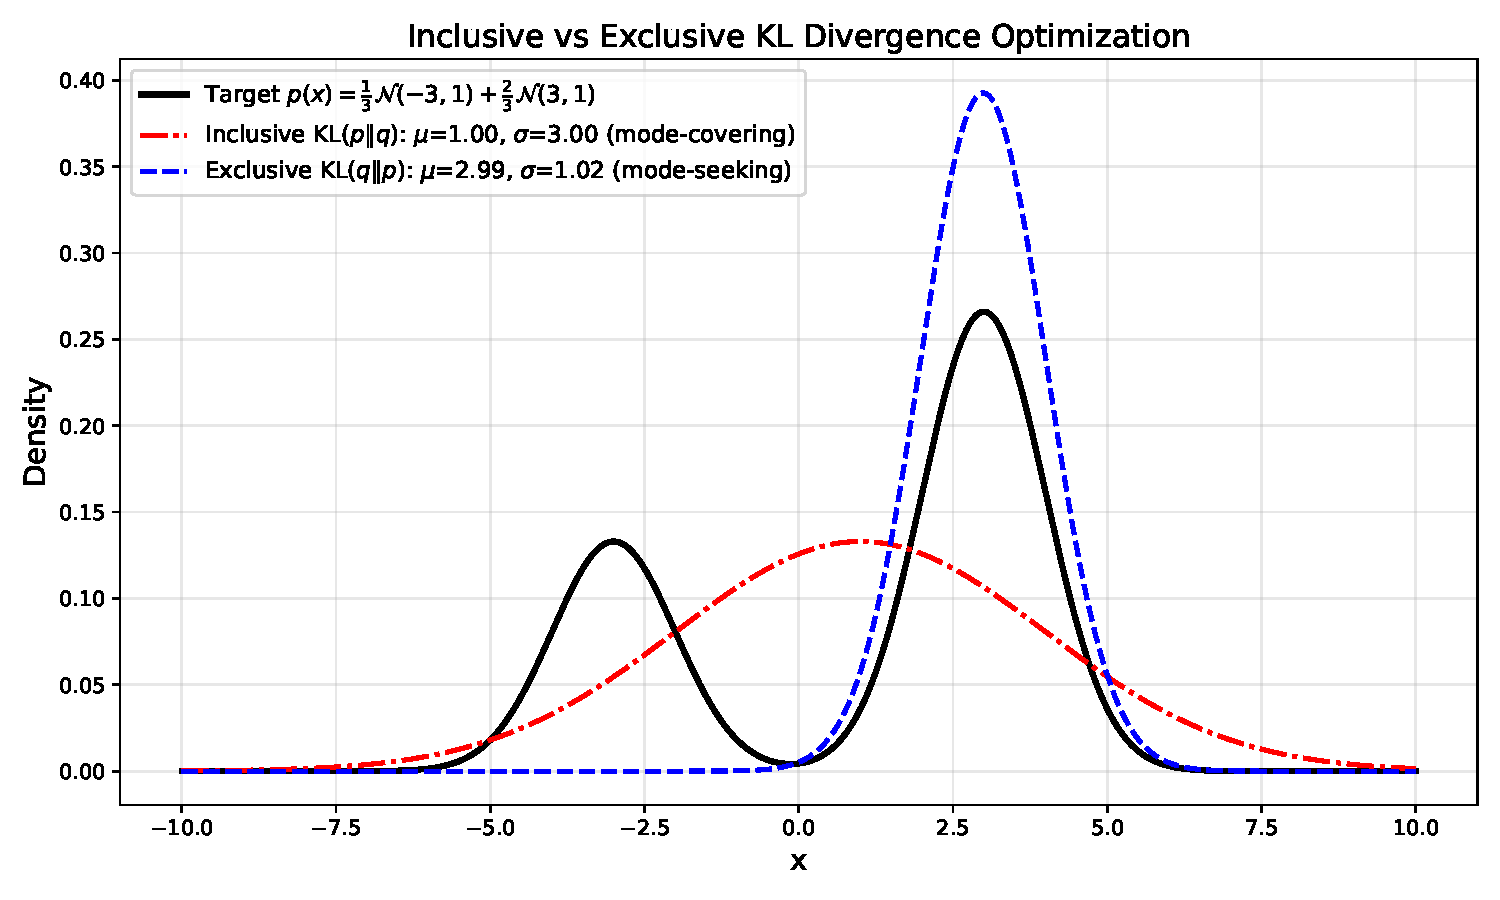
\includegraphics[width=0.85\textwidth]{kl_divergence.pdf}
            \caption{Comparison of inclusive and exclusive KL divergence optimization. The inclusive KL ($\mathrm{KL}(p\|q)$, mode-covering) produces a broad distribution that covers all modes, while the exclusive KL ($\mathrm{KL}(q\|p)$, mode-seeking) concentrates on the dominant mode.}
            \label{fig:kl}
        \end{figure}

        The Python code used to generate this figure is provided in the accompanying file \texttt{kl\_divergence.py}.

        \item \textbf{(Variational Inference with Forward KL)}

        Bob proposes using the forward KL-divergence $\mathrm{KL}(p(z|x) \| q_\psi(z|x))$.

        Expanding:
        \begin{align}
        \mathrm{KL}(p(z|x) \| q_\psi(z|x))
        &= \mathbb{E}_{z \sim p(z|x)}\left[\log \frac{p(z|x)}{q_\psi(z|x)}\right] \nonumber \\
        &= \mathbb{E}_{z \sim p(z|x)}[\log p(z|x)] - \mathbb{E}_{z \sim p(z|x)}[\log q_\psi(z|x)]. \nonumber
        \end{align}

        Since $\mathbb{E}_{z \sim p(z|x)}[\log p(z|x)]$ does not depend on $\psi$, minimizing over $\psi$ is equivalent to:
        \[
        \max_\psi \; \mathbb{E}_{z \sim p(z|x)}[\log q_\psi(z|x)].
        \]

        This is the objective for $q_\psi(z|x)$: maximize the expected log-likelihood of $q_\psi$ under the true posterior.

        \textbf{Pros:}
        \begin{itemize}
            \item The forward KL is \emph{mode-covering} (inclusive): $q_\psi(z|x)$ will try to cover all modes of $p(z|x)$, avoiding mode collapse. This can lead to a more faithful approximation of the full posterior.
            \item If the true posterior is multi-modal, forward KL will not miss modes.
        \end{itemize}

        \textbf{Cons:}
        \begin{itemize}
            \item The objective requires sampling from the true posterior $p(z|x)$, which is intractable in VAE --- this is the very distribution we are trying to approximate. Thus, this objective \emph{cannot be directly optimized} in the VAE framework without additional techniques (e.g., importance sampling, MCMC).
            \item Because forward KL is mode-covering, $q_\psi(z|x)$ may spread probability mass over regions where $p(z|x)$ is negligible, leading to a high-variance, overly diffuse approximation.
            \item It cannot be incorporated into the standard ELBO framework, which naturally arises from the reverse KL.
        \end{itemize}
    \end{enumerate}
}

%% Problem 7 (GM-VAE)
\solution{
    \begin{enumerate}
        \item \textbf{ELBO Derivation}

        We derive the ELBO for $\log p_{\mu,\sigma,\theta}(x)$.

        \begin{align}
        \log p(x) &= \log \sum_z \int p(x, w, z) \, dw \nonumber \\
        &= \log \sum_z \int \frac{q_{\psi,\phi}(w,z|x)}{q_{\psi,\phi}(w,z|x)} p(x,w,z) \, dw \nonumber \\
        &\geq \mathbb{E}_{(w,z) \sim q_{\psi,\phi}(w,z|x)} \left[ \log \frac{p(x,w,z)}{q_{\psi,\phi}(w,z|x)} \right] \quad \text{(by Jensen's inequality)} \nonumber
        \end{align}

        Now expand $p(x,w,z) = p(z) \, p_{\mu,\sigma}(w|z) \, p_\theta(x|w)$ and $q_{\psi,\phi}(w,z|x) = q_\psi(w|x) \, q_\phi(z|w,x)$:

        \begin{align}
        \mathrm{ELBO} &= \mathbb{E}_{q_\psi(w|x) q_\phi(z|w,x)} \left[ \log \frac{p(z) \, p_{\mu,\sigma}(w|z) \, p_\theta(x|w)}{q_\psi(w|x) \, q_\phi(z|w,x)} \right] \nonumber \\
        &= \mathbb{E}_{q_\psi(w|x) q_\phi(z|w,x)} \left[ \log p_\theta(x|w) + \log \frac{p_{\mu,\sigma}(w|z)}{q_\psi(w|x)} + \log \frac{p(z)}{q_\phi(z|w,x)} \right] \nonumber
        \end{align}

        Separating the three terms:

        \begin{align}
        \mathrm{ELBO} &= \underbrace{\mathbb{E}_{q_\psi(w|x)}[\log p_\theta(x|w)]}_{\text{Reconstruction}} \nonumber \\
        &\quad + \underbrace{\mathbb{E}_{q_\psi(w|x) q_\phi(z|w,x)}\left[\log \frac{p_{\mu,\sigma}(w|z)}{q_\psi(w|x)}\right]}_{\text{Latent } w \text{ regularization}} \nonumber \\
        &\quad + \underbrace{\mathbb{E}_{q_\psi(w|x) q_\phi(z|w,x)}\left[\log \frac{p(z)}{q_\phi(z|w,x)}\right]}_{\text{Latent } z \text{ regularization}} \nonumber
        \end{align}

        The three terms can be interpreted as follows:
        \begin{itemize}
            \item \textbf{Term 1} (involving $p_\theta(x|w)$): Reconstruction term --- measures how well the decoder reconstructs $x$ from latent $w$.
            \item \textbf{Term 2} (involving $p_{\mu,\sigma}(w|z)$): Can be rewritten as $-\mathbb{E}_{q_\phi(z|w,x)}[\mathrm{KL}(q_\psi(w|x) \| p_{\mu,\sigma}(w|z))]$ --- regularizes the encoder $q_\psi(w|x)$ to match the Gaussian mixture component $p_{\mu,\sigma}(w|z)$.
            \item \textbf{Term 3} (involving $p(z)$): Equals $-\mathbb{E}_{q_\psi(w|x)}[\mathrm{KL}(q_\phi(z|w,x) \| p(z))]$ --- regularizes the cluster assignment $q_\phi(z|w,x)$ to match the prior $p(z)$.
        \end{itemize}

        \item \textbf{Training Procedure for GM-VAE}

        \begin{enumerate}
            \item \textbf{Network Architecture:}
            \begin{itemize}
                \item \textbf{Encoder} $q_\psi(w|x)$: A neural network that takes $x$ as input and outputs the mean $\mu_\psi(x)$ and variance $\sigma^2_\psi(x)$ of a Gaussian distribution over $w$. Use the reparameterization trick: $w = \mu_\psi(x) + \sigma_\psi(x) \odot \epsilon$, $\epsilon \sim \mathcal{N}(0,I)$.
                \item \textbf{Cluster inference network} $q_\phi(z|w,x)$: A neural network that takes $w$ and $x$ as input and outputs a categorical distribution over $z \in \{1,\ldots,K\}$ (softmax output).
                \item \textbf{Decoder} $p_\theta(x|w)$: A neural network that takes $w$ as input and outputs the mean $\mu_\theta(w)$ and variance $\sigma^2_\theta(w)$ of a Gaussian distribution over $x$.
                \item \textbf{Learnable prior parameters}: $\mu_k, \sigma_k$ for $k=1,\ldots,K$ (means and standard deviations of each Gaussian component).
            \end{itemize}

            \item \textbf{Training Loop} (for each mini-batch of data $\{x^{(i)}\}$):
            \begin{enumerate}
                \item \textbf{Encode}: For each $x^{(i)}$, compute $\mu_\psi(x^{(i)})$ and $\sigma_\psi(x^{(i)})$, sample $w^{(i)} = \mu_\psi(x^{(i)}) + \sigma_\psi(x^{(i)}) \odot \epsilon^{(i)}$ via reparameterization.
                \item \textbf{Cluster Assignment}: Compute $q_\phi(z=k|w^{(i)}, x^{(i)})$ for each $k = 1,\ldots,K$.
                \item \textbf{Decode}: Compute $\mu_\theta(w^{(i)})$ and $\sigma^2_\theta(w^{(i)})$ to evaluate $\log p_\theta(x^{(i)}|w^{(i)})$.
                \item \textbf{Compute ELBO}: Evaluate the three ELBO terms:
                \begin{itemize}
                    \item Reconstruction: $\log p_\theta(x^{(i)}|w^{(i)})$.
                    \item $w$-regularization: $\sum_k q_\phi(z=k|w^{(i)},x^{(i)}) \log \frac{p_{\mu_k,\sigma_k}(w^{(i)}|z=k)}{q_\psi(w^{(i)}|x^{(i)})}$.
                    \item $z$-regularization: $\sum_k q_\phi(z=k|w^{(i)},x^{(i)}) \log \frac{p(z=k)}{q_\phi(z=k|w^{(i)},x^{(i)})}$.
                \end{itemize}
                \item \textbf{Update}: Maximize the ELBO using gradient ascent (or equivalently, minimize $-$ELBO) with respect to all parameters $\theta, \psi, \phi, \mu, \sigma$ using Adam or SGD.
            \end{enumerate}

            \item \textbf{Key Implementation Details:}
            \begin{itemize}
                \item Use the reparameterization trick for $w$ to enable backpropagation through sampling.
                \item For the discrete variable $z$, use the Gumbel-Softmax trick or marginalize over $z$ analytically (since $z$ is discrete with $K$ values, we can enumerate all $K$ components).
                \item The KL term for $z$ can be computed in closed form as the KL between a categorical and a uniform distribution.
            \end{itemize}
        \end{enumerate}
    \end{enumerate}
}

%% Problem 8 (AI Usage)
\solution{
    Used Claude (AI assistant by Anthropic) in the following capacities:
    \begin{itemize}
        \item \textbf{Solution ideation:} Brainstorming approaches and generating initial ideas for problem-solving strategies, particularly for structuring mathematical proofs and derivations.
        \item \textbf{English grammar and writing:} Polishing and refining the English writing throughout the solutions to improve clarity, coherence, and academic tone.
        \item \textbf{\LaTeX{} formatting:} Optimizing typesetting and layout of mathematical expressions, tables, and document structure for better readability and presentation.
        \item \textbf{Result verification:} Cross-checking the correctness of intermediate computations, final answers, and logical consistency of proofs.
    \end{itemize}
    All final solutions were reviewed and verified by the author.
}

\ifnum\value{placeholderCount}>0
    \vfill
    \begin{center}
        \color{red} \framebox{\textbf{WARNING: PLEASE REMOVE ALL PLACEHOLDERS BEFORE SUBMISSION}}
    \end{center}
\fi

\end{document}
